%%%%%%%%%%%%%%%%%%%%%%%%%%%%%%%%%%%%%%%%%%%%%%%%%%%%%%%%%%%%%%%%%
%
% Project     : Bachelorarbeit
% Title       : Machbarkeitsanalyse für eine ressourcenorientierte Schnittstelle zur Verarbeitung grundlegender Probleme der Informatik
% File        : anforderungsdokument.tex Rev. 01
% Date        : 01.03.2015
% Author      : Raffael Santschi
%
%%%%%%%%%%%%%%%%%%%%%%%%%%%%%%%%%%%%%%%%%%%%%%%%%%%%%%%%%%%%%%%%%

\chapter{Anforderungsdokument \resultAssignment{[R3]}}\label{chap.anforderungsdokument}

Das Anforderungsdokument legt die Basis für die Implementation. Es ist für den Verlauf des Projekts wichtig, dass zu Beginn die Anforderungen aufgestellt werden. Bei der 
Erstellung des Anforderungsdokuments werden verschiedene Betrachtungsweisen aufgezeigt und die Herausforderung in verschiedenen Detailstufen angeschaut.


\section{Übersicht}\label{anf_uebersicht}

In diesem Abschnitt  wird die System- und Kontextabgrenzung dargelegt, die Systemumgebung beschrieben, die getroffenen Annahmen festgehalten und die verschiedenen \gls{stakeholder} mit 
ihren Erwartungen aufgelistet.

\subsection{System- und Kontextabgrenzung}\label{systemabgrenzung}
Der Systemkontext umfasst alle Aspekte, die für die Anforderungen des geplanten Systems relevant sind und nicht im Rahmen der Entwicklung dieses System gestaltet werden können.
\cite{req_eng_book} 

\begin{figure}[h]
\centering
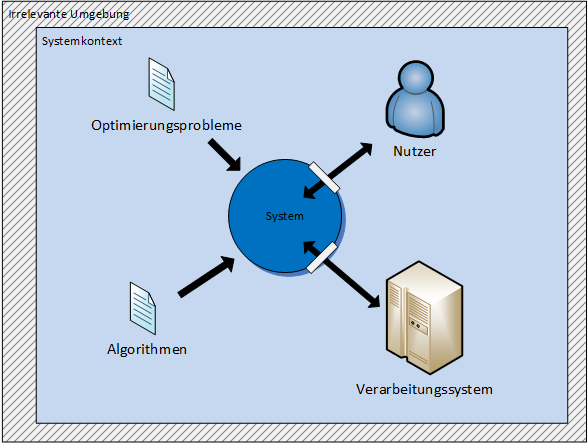
\includegraphics[scale=0.8]{images/visio/systemkontext.png}
\caption[Systemkontext]{Systemkontext \selfmade{}}
\label{fig:systemkontext}
\end{figure}

Der Systemkontext (siehe Abbildung \ref{fig:systemkontext}) zeigt, dass das System eine relevanten Schnittstellen zu den Nutzern und Verarbeitungssystem hat. Das System muss Daten für 
das Verarbeitungssystem zur Verfügung stellen und auch solche annehmen. Des weiteren wird das System von den Nutzern, Optimierungsproblemen und den dazugehörigen Algorithmen 
beeinflusst.

\FloatBarrier
\subsection{Systemumgebung}\label{systemumgebung}
Die Systemumgebung (siehe Abbildung \ref{fig:systemumgebung}) definiert die Ausgangslage für das Projekt. Am Anfang des Projekts war bekannt, dass Nutzer und ein Verarbeitungssystem 
Dienste des zu erstellendem System beziehen wollen. Die genaue Ausprägung dieser Dienste werden in diesem Kapitel behandelt.

\begin{figure}[h]
\centering
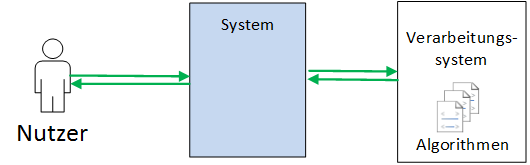
\includegraphics[scale=0.8]{images/visio/systemumgebung.png}
\caption[Systemumgebung]{Systemumgebung \selfmade{}}
\label{fig:systemumgebung}
\end{figure}

\FloatBarrier
\subsection{Annahmen}\label{annahmen}
Zwischen dem Endnutzer und dem zu erstellenden System existiert noch ein Sicherheitslayer, welcher nicht Teil dieser Arbeit ist. Später wird dieses Projekt allenfalls mit diesem Sicherheitslayer 
erweitert oder eine übergeordnete Schnittstellen erstellt, welche diese anspricht. 

Je nach Algorithmus Implementation, ist das Ansteuern und die Aufbereitung der Daten unterschiedlich. Eine Referenzimplementierung zu jedem Problem zu finden, stellte sich als schwierig 
heraus. Deshalb wurden die Ein- und Ausgabe Schemas der Algorithmen aus den Literaturrecherchen abgeleitet.

\newpage
\subsection{Stakeholder}\label{stakeholder}
Die \gls{stakeholder} Analyse dient dem erfassen aller Nutzergruppen, die auf ein Projekt Einfluss haben. Zudem ermöglicht sie die Erfassung aller Gruppen, die potentiell 
Anforderungen an das Projekt stellen. In der der Tabelle \ref{table:stakeholder} wurden die \gls{stakeholder} für dieses Projekt zusammengetragen und ihre Erwartungen, ihre 
Einstellung und ihr Einfluss gegenüber diesem Projekt festgehalten. Da dieses Projekt eine Machbarkeitsanalyse ist, befindet sich nur der Auftraggeber und ein potenzieller Kunde in der 
Auflistung.

\begin{table}[ht]
\centering
  \begin{tabular}{ p{5cm} | p{5cm} | p{1.5cm} | p{1.5cm} }
	\hline
	\rowcolor{darkgray}
	\textbf{Name}					&	\textbf{Erwartung}	&	\textbf{Einstellung} 	&	\textbf{Einfluss}	\\ \hline
	\rowcolor{gray}
								&				&	-Positiv \mbox{-Neutral} \mbox{-Negativ} 	&	-Hoch \mbox{-Mittel} \mbox{-Niedrig} \\ \hline
	\textbf{Phil Hofmann} (Vorsteher der Geschäftsführung der 200ok GmbH)						
								&	Phil ist der Auftraggeber in diesem Projekt. Er erwartet von der Machbarkeitsanalyse Informationen für ein mögliches Projekt zur 
									Umsetzung der Gesamtidee.
												& 	Positiv		&	Hoch		\\ \hline
	\textbf{Potenzieller Kunde}
								&	Der potenzielle Kunde wünscht sich eine einfache Abwicklung für seine Probleme, er möchte sich nicht mit Algorithmen und 
									theoretischer Informatik rumschlagen.
												& 	Positiv		&	Hoch		\\ \hline
  \end{tabular}
   \caption{Liste der \gls{stakeholder}}\label{table:stakeholder}
\end{table}

\newpage
\section{Anforderungen}\label{sec.anfoderungen}
Beim Erfassen der Anforderungen wurden zuerst die Use-Cases definiert. Anhand der Use-Cases wurden die Anforderungen abgeleitet.

\subsection{Use Cases}\label{use_cases}
Das Use Case Diagramm (siehe Abbildung \ref{fig:use_case}) zeigt einen Akteur, ein System und sechs Use Cases, welche für diese Arbeit relevant sind.
\begin{figure}[h]
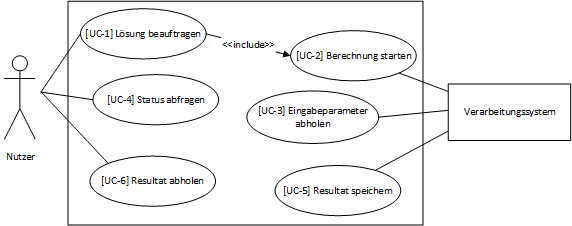
\includegraphics{images/anforderungen/use_cases.png}
\caption[Use-Case Diagramm]{Use-Case Diagramm \selfmade{}}
\label{fig:use_case}
\end{figure}

Alle Use Cases wurden anhand der folgenden Vorlage (siehe Tabelle \ref{table:use_case_template}) spezifiziert. Diese Vorlage basiert auf Angaben von \cite{req_eng_book}.

\begin{table}[ht]
\centering
  \begin{tabular}{ l | p{10cm} }
	\hline
	\rowcolor{gray}
	\textbf{Bezeichner}&	\textbf{Eindeutiger Bezeichner}\\ \hline
	\textbf{Name}		&	Eindeutiger Name\\ \hline
	\textbf{Beschreibung}	&	Komprimierte Beschreibung\\ \hline
	\textbf{Auslösendes Ereignis} &	Angabe des Ereignisses, das den Use Case auslöst\\ \hline
	\textbf{Akteure}		&	Auflistung der Akteure, die mit dem Use Case in Beziehung stehen\\ \hline
	\textbf{Vorbedingung}	&	Eine Liste notwendiger Voraussetzungen, die erfüllt sein müssen, bevor die Ausführung des Use Case beginnen kann\\ \hline
	\textbf{Nachbedingung}	&	Eine Liste von Zuständen, in denen sich das System unmittelbar nach der Ausführung des Hauptszenarios befindet.\\ \hline
	\textbf{Ergebnis}		&	Beschreibung der Ausgaben, die während der Ausführung des Use Case erzeugt werden\\ \hline
	\textbf{Hauptszenario}	&	Beschreibung des Hauptszenarios eines Use Case\\ \hline
	\textbf{Alternativszenarien}	&	Beschreibung von Alternativszenarien des Use Case oder lediglich Angabe der auslösenden Ereignisse. 
					Hier gelten oftmals andere Nachbedingungen.\\ \hline
  \end{tabular}
   \caption{Vorlage für Use Case Spezifikation}\label{table:use_case_template}
\end{table}

\begin{table}[ht]
\centering
  \begin{tabular}{ l | p{10cm} }
	\hline
	\rowcolor{gray}
	\textbf{Bezeichner}	&	\textbf{UC-1}\\ \hline
	\textbf{Name}		&	Lösung beauftragen\\ \hline
	\textbf{Beschreibung}	&	Ein Nutzer möchte eine Lösung eines Problem mit spezifischen Parametern beauftragen.\\ \hline
	\textbf{Auslösendes Ereignis} &	Nutzer möchte ein Problem lösen.\\ \hline
	\textbf{Akteure}		&	Nutzer\\ \hline
	\textbf{Vorbedingung}	&	Das System bietet zur Lösung dieses Problems einen Aufruf.\\ \hline
	\textbf{Nachbedingung}	&	Das System hat die nötigen Informationen für die Lösung des Problems und der Nutzer erhält eine ID, mit welcher er den Status bzw. das Resultat 
						abholen kann.\\ \hline
	\textbf{Ergebnis}		&	Erfassung der Informationen für die Lösung des Problems\\ \hline
	\textbf{Hauptszenario}	&	\begin{enumerate}
					\item Der Nutzer ruft die Funktion für das zu lösende Problem mit den Parametern auf.
					\item Das System speichert die Parameter für die weitere Verarbeitung.
					\item Der Nutzer erhält eine ID für das Abrufen des Status bzw. des Resultates.
					\end{enumerate}
					\\ \hline
	\textbf{Alternativszenarien}	&	\begin{enumerate}
					\item[3a] Der Nutzer erhält eine Fehlermeldung, wenn das Problem nicht korrekt erfasst werden konnte.
					\end{enumerate}
					\\ \hline
  \end{tabular}
   \caption{Use Case UC-1: Lösung beauftragen}\label{table:use_case_1}
\end{table}

\begin{table}[ht]
\centering
  \begin{tabular}{ l | p{10cm} }
	\hline
	\rowcolor{gray}
	\textbf{Bezeichner}	&	\textbf{UC-2}\\ \hline
	\textbf{Name}			&	Berechnung starten\\ \hline
	\textbf{Beschreibung}	&	Das System startet die Berechnung beim Verarbeitungssystem.\\ \hline
	\textbf{Auslösendes Ereignis} &	Nutzer möchte ein Problem lösen.\\ \hline
	\textbf{Akteure}		&	Verarbeitungssystem\\ \hline
	\textbf{Vorbedingung}	&	Die Informationen für die Lösung des Problems sind erfasst.\\ \hline
	\textbf{Nachbedingung}	&	Das Verarbeitungssystem beginnt mit der Berechnung.\\ \hline
	\textbf{Ergebnis}		&	Starten der Berechnung\\ \hline
	\textbf{Hauptszenario}	&	\begin{enumerate}
					\item Das System startet die Berechnung. 
					\item Das System übergibt eine ID für das Abrufen der abgelegten Daten.
					\end{enumerate}
					\\ \hline
	\textbf{Alternativszenarien}	&	\begin{enumerate}
					\item[2a] Das System speichert die Fehlermeldung, falls das Starten der Berechnung fehlschlägt.
					\end{enumerate}
					\\ \hline
  \end{tabular}
   \caption{Use Case UC-2: Berechnung starten}\label{table:use_case_2}
\end{table}

\begin{table}[ht]
\centering
  \begin{tabular}{ l | p{10cm} }
	\hline
	\rowcolor{gray}
	\textbf{Bezeichner}	&	\textbf{UC-3}\\ \hline
	\textbf{Name}			&	Eingabe Parameter abholen\\ \hline
	\textbf{Beschreibung}	&	Das Verarbeitungssystem benötigt für die Lösung des Problems die Eingabeparameter.\\ \hline
	\textbf{Auslösendes Ereignis}&	Das Verarbeitungssystem möchte die Eingabeparameter.\\ \hline
	\textbf{Akteure}		&	Verarbeitungssystem\\ \hline
	\textbf{Vorbedingung}	&	Das Verarbeitungssystem wurden angestossen das Problem zu lösen.\\ \hline
	\textbf{Nachbedingung}	&	Das Verarbeitungssystem hat die Eingabeparameter erhalten.\\ \hline
	\textbf{Ergebnis}		&	Erhalt von Eingabeparametern\\ \hline
	\textbf{Hauptszenario}	&	\begin{enumerate}
					\item Das Verarbeitungssystem fordert die Eingabeparameter für das zu lösende Problem an.
					\item Das System leitet die Eingabeparameter weiter.
					\item Das Verarbeitungssystem erhält die Eingabeparameter.
					\end{enumerate}
					\\ \hline
	\textbf{Alternativszenarien}	&	\begin{enumerate}
					\item[2a] Das System sendet eine Fehlermeldung, falls keine Eingabeparameter vorhanden sind.
					\end{enumerate}
					\\ \hline
  \end{tabular}
   \caption{Use Case UC-3: Eingabe Parameter abholen}\label{table:use_case_3}
\end{table}


\begin{table}[ht]
\centering
  \begin{tabular}{ l | p{10cm} }
	\hline
	\rowcolor{gray}
	\textbf{Bezeichner}	&	\textbf{UC-4}\\ \hline
	\textbf{Name}			&	Status abfragen\\ \hline
	\textbf{Beschreibung}	&	Der Nutzer kann den Status einer Berechnung abfragen, da die Verarbeitung einige Zeit benötigt.\\ \hline
	\textbf{Auslösendes Ereignis}&	Der Nutzer möchte den Status der Berechnung wissen.\\ \hline
	\textbf{Akteure}		&	Nutzer\\ \hline
	\textbf{Vorbedingung}	&	Der Nutzer hat bereits eine Berechnung beauftragt und kennt die ID.\\ \hline
	\textbf{Nachbedingung}	&	Der Nutzer kennt den Status der Berechnung.\\ \hline
	\textbf{Ergebnis}		&	Kenntnis des Status\\ \hline
	\textbf{Hauptszenario}	&	\begin{enumerate}
					\item Der Nutzer fragt den Status einer Berechnung ab.
					\item Das System fragt den Status ab.
					\item Das System sendet den Status zurück.
					\item Der Nutzer erhält den Status.
					\end{enumerate}
					\\ \hline
	\textbf{Alternativszenarien}	&	\begin{enumerate}
					\item[3a] Das System sendet eine Fehlermeldung zurück, falls der Status nicht ermittelt werden kann.
					\end{enumerate}
					\\ \hline
  \end{tabular}
   \caption{Use Case UC-4: Status abfragen}\label{table:use_case_4}
\end{table}

\begin{table}[ht]
\centering
  \begin{tabular}{ l | p{10cm} }
	\hline
	\rowcolor{gray}
	\textbf{Bezeichner}	&	\textbf{UC-5}\\ \hline
	\textbf{Name}			&	Resultat speichern\\ \hline
	\textbf{Beschreibung}	&	Da die Aufrufe asynchron sind, muss das Ergebnis nach der Berechnung zwischengespeichert werden.\\ \hline
	\textbf{Auslösendes Ereignis}&	Das Verarbeitungssystem möchte das Resultat speichern.\\ \hline
	\textbf{Akteure}		&	Verarbeitungssystem\\ \hline
	\textbf{Vorbedingung}	&	Das Verarbeitungssystem hat ein Resultat berechnet.\\ \hline
	\textbf{Nachbedingung}	&	Das Resultat ist gespeichert.\\ \hline
	\textbf{Ergebnis}		&	Speicherung des Resultats\\ \hline
	\textbf{Hauptszenario}	&	\begin{enumerate}
					\item Das Verarbeitungssystem schickt das Resultat der Berechnung dem System.
					\item Das System erhält das Resultat.
					\item Das System speichert das Resultat.
					\item Das System quittiert das Erhalten des Resultats.
					\item Das Verarbeitungssystem erhält die Bestätigung.
					\end{enumerate}
					\\ \hline
	\textbf{Alternativszenarien}	&	\begin{enumerate}
					\item[4a] Das System sendet eine Fehlermeldung, wenn das Resultat nicht korrekt gespeichert werden konnte.
					\end{enumerate}
					\\ \hline
  \end{tabular}
   \caption{Use Case UC-5: Resultat speichern}\label{table:use_case_5}
\end{table}

\begin{table}[ht]
\centering
  \begin{tabular}{ l | p{10cm} }
	\hline
	\rowcolor{gray}
	\textbf{Bezeichner}	&	\textbf{UC-6}\\ \hline
	\textbf{Name}			&	Resultat abholen\\ \hline
	\textbf{Beschreibung}	&	Der Nutzer holt das Resultat an einem bestimmten Zeitpunkt ab.\\ \hline
	\textbf{Auslösendes Ereignis}&	Der Nutzer möchte das Resultat der Berechnung abholen.\\ \hline
	\textbf{Akteure}		&	Nutzer\\ \hline
	\textbf{Vorbedingung}	&	Der Nutzer hat bereits eine Berechnung beauftragt und kennt die ID.\\ \hline
	\textbf{Nachbedingung}	&	Der Nutzer hat das Resultat erhalten.\\ \hline
	\textbf{Ergebnis}		&	Erhalt des Resultats\\ \hline
	\textbf{Hauptszenario}	&	\begin{enumerate}
					\item Der Nutzer ruft das Resultat der Berechnung ab.
					\item Das System sucht das Resultat der Berechnung.
					\item Das System sendet das Resultat.
					\item Der Nutzer erhält das Resultat.
					\end{enumerate}
					\\ \hline
	\textbf{Alternativszenarien}	&	\begin{enumerate}
					\item[3a] Das System sendet eine Fehlermeldung, wenn kein Resultat vorhanden ist.
					\end{enumerate}
					\\ \hline
  \end{tabular}
   \caption{Use Case UC-6: Resultat abholen}\label{table:use_case_6}
\end{table}

\newpage
\FloatBarrier
\subsection{Anforderungen}\label{anforderungen}
Alle Anforderungen wurden anhand der folgenden Vorlage (siehe Tabelle \ref{table:req_template}) erfasst. Diese Vorlage basiert auf Angaben von \cite{req_eng_book} und wurde mit 
eigenen Attributen erweitert.

\begin{table}[ht]
\centering
  \begin{tabular}{ l | p{8cm} }
	\hline
	\rowcolor{gray}
	\textbf{Bezeichner}&	\textbf{Eindeutiger Identifikator}\\ \hline
	\textbf{Priorität} 		&	Must, Should, Nice to have\\ \hline
	\textbf{Anforderungstyp}	&	Funktionale Anforderung, Qualitätsanforderung, Randbedingung\\ \hline
	\textbf{Name} 			&	Eindeutiger, charakterisierender Name\\ \hline
	\textbf{Use Case} 		&	Referenz zum zugehörigen Use Case\\ \hline
	\textbf{Beschreibung} 	&	Beschreibung der Anforderung\\ \hline
	\textbf{Begründung} 		&	Bedeutung der Anforderung für das geplante System\\ \hline
	\textbf{Akzeptanz Kriterium}	&	Messbare Abnahmekriterien\\ \hline
	\textbf{Abhängigkeiten} 	&	Referenz zu anderen Anforderungen\\ \hline
  \end{tabular}
   \caption{Vorlage für Anforderungen}\label{table:req_template}
\end{table}


Die Beschreibung der Anforderungen wurden zusätzlich mit der Satzschablone in \autoref{fig:satzschablone}) aus \cite{req_eng_book} erstellt. Dies hat den Vorteil, dass die 
Anforderungen normiert und exakt daherkommen. Die Abstufungen \textit{muss}, \textit{sollte} und \textit{wird} werden verwendet, um die Wichtigkeit der Anforderungen auszudrücken.
\begin{figure}[h]
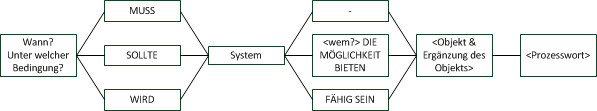
\includegraphics[scale=0.95]{images/anforderungen/satzschablone.png}
\caption[Satzschablone]{Satzschablone (Grafik entnommen aus \cite{req_eng_book})}
\label{fig:satzschablone}
\end{figure}


\newpage
\FloatBarrier
\subsubsection{Funktionale Anforderungen}\label{func_anforderungen}

\begin{table}[ht]
\centering
  \begin{tabular}{ l | p{8cm} }
	\hline
	\rowcolor{gray}
	\textbf{Bezeichner}&	\textbf{RE-F1}\\ \hline
	\textbf{Priorität} 		&	Must\\ \hline
	\textbf{Anforderungstyp}	&	Funktionale Anforderung\\ \hline
	\textbf{Name} 			&	Bereitstellung der Schnittstellen für Optimierungsprobleme\\ \hline
	\textbf{Use Case} 		&	\nameref{table:use_case_1}\\ \hline
	\textbf{Beschreibung} 	&	Das System muss dem Nutzer die Möglichkeit bieten, die Lösung verschiedener Optimierungsprobleme zu beauftragen.\\ \hline
	\textbf{Begründung} 		&	Die Schnittstellen ist die Anlaufstelle des Nutzers. Er beauftragt das System, eine Berechnung zu starten.\\ \hline
	\textbf{Akzeptanz Kriterium}	&	\begin{enumerate}
					\item Der Nutzer kann eine Schnittstelle für eine bereitgestellten Berechnungsfunktionen ansprechen.
					\end{enumerate}
					\\ \hline
	\textbf{Abhängigkeiten} 	&	-\\ \hline
  \end{tabular}
   \caption{Anforderung RF-F1}\label{table:req_1}
\end{table}

\begin{table}[ht]
\centering
  \begin{tabular}{ l | p{8cm} }
	\hline
	\rowcolor{gray}
	\textbf{Bezeichner}&	\textbf{RE-F2}\\ \hline
	\textbf{Priorität} 		&	Must\\ \hline
	\textbf{Anforderungstyp}	&	Funktionale Anforderung\\ \hline
	\textbf{Name} 			&	Speicherung der Eingabeparameter\\ \hline
	\textbf{Use Case} 		&	\nameref{table:use_case_1}\\ \hline
	\textbf{Beschreibung} 	&	Falls eine Berechnung in Auftrag gegeben wurde, muss das System fähig sein, die Eingabeparameter abzuspeichern.\\ \hline
	\textbf{Begründung} 		&	Die Berechnung wird von einem anderen System ausgeführt, damit dieses auf die Parameter zu greifen kann, müssen sie persistiert werden.\\ \hline
	\textbf{Akzeptanz Kriterium}	&	\begin{enumerate}
					\item Die Parameter sind persistiert.
					\item Es gibt eine Fehlermeldung, falls bei der Speicherung etwas fehlschlägt oder die Eingabeparameter nicht gültig sind.
					\end{enumerate}
					\\ \hline
	\textbf{Abhängigkeiten} 	&	\\ \hline
  \end{tabular}
   \caption{Anforderung RF-F2}\label{table:req_3}
\end{table}

\begin{table}[ht]
\centering
  \begin{tabular}{ l | p{8cm} }
	\hline
	\rowcolor{gray}
	\textbf{Bezeichner}&	\textbf{RE-F3}\\ \hline
	\textbf{Priorität} 		&	Must\\ \hline
	\textbf{Anforderungstyp}	&	Funktionale Anforderung\\ \hline
	\textbf{Name} 			&	Rückgabe einer ID bei Beauftragung\\ \hline
	\textbf{Use Case} 		&	\nameref{table:use_case_1}\\ \hline
	\textbf{Beschreibung} 	&	Falls eine Berechnung in Auftrag gegeben wurde, muss das System dem Ersteller eine ID zurückliefern.\\ \hline
	\textbf{Begründung} 		&	Die ID hilft dem Nutzer den Status der Berechnung abzuholen und wird am Schluss für das Resultat benötigt.\\ \hline
	\textbf{Akzeptanz Kriterium}	&	\begin{enumerate}
					\item Der Nutzer erhält nach dem Starten einer Berechnung eine ID.
					\end{enumerate}
					\\ \hline
	\textbf{Abhängigkeiten} 	&	\nameref{table:req_3}\\ \hline
  \end{tabular}
   \caption{Anforderung RF-F3}\label{table:req_2}
\end{table}

\begin{table}[ht]
\centering
  \begin{tabular}{ l | p{8cm} }
	\hline
	\rowcolor{gray}
	\textbf{Bezeichner}&	\textbf{RE-F4}\\ \hline
	\textbf{Priorität} 		&	Must\\ \hline
	\textbf{Anforderungstyp}	&	Funktionale Anforderung\\ \hline
	\textbf{Name} 			&	Start der Berechnung\\ \hline
	\textbf{Use Case} 		&	\nameref{table:use_case_2}\\ \hline
	\textbf{Beschreibung} 	&	Falls eine Berechnung in Auftrag gegeben wurde, muss das System fähig sein, die Berechnung beim Verarbeitungssystem zu starten.\\ \hline
	\textbf{Begründung} 		&	Der Nutzer kennt das Verarbeitungssystem nicht, das System muss dem Verarbeitungssystem den Start Befehl geben.\\ \hline
	\textbf{Akzeptanz Kriterium}	&	\begin{enumerate}
					\item Der Befehl für den Start wird versendet und die ID dabei übergeben.
					\item Die Fehlermeldung bei einem Fehlversuch wird gespeichert.
					\end{enumerate}
					\\ \hline
	\textbf{Abhängigkeiten} 	&	\nameref{table:req_3}\\ \hline
  \end{tabular}
   \caption{Anforderung RF-F4}\label{table:req_4}
\end{table}

\begin{table}[ht]
\centering
  \begin{tabular}{ l | p{8cm} }
	\hline
	\rowcolor{gray}
	\textbf{Bezeichner}&	\textbf{RE-F5}\\ \hline
	\textbf{Priorität} 		&	Must\\ \hline
	\textbf{Anforderungstyp}	&	Funktionale Anforderung\\ \hline
	\textbf{Name} 			&	Abfrage der Eingabeparameter\\ \hline
	\textbf{Use Case} 		&	\nameref{table:use_case_3}\\ \hline
	\textbf{Beschreibung} 	&	Falls eine Berechnung in Auftrag gegeben wurde, muss das System dem Verarbeitungssystem die Möglichkeit bieten, die Eingabeparameter abzufragen.\\ \hline
	\textbf{Begründung}		&	Damit das Verarbeitungssystem die Berechnung durchführen kann, braucht es die Eingabeparameter.\\ \hline
	\textbf{Akzeptanz Kriterium}	&	\begin{enumerate}
					\item Das Verarbeitungssystem erhält die Eingabeparameter.
					\item Das Verarbeitungssystem erhält eine Fehlermeldung, falls keine Eingabeparameter vorhanden sind.
					\end{enumerate}
					\\ \hline
	\textbf{Abhängigkeiten} 	&	\nameref{table:req_3}\\ \hline
  \end{tabular}
   \caption{Anforderung RF-F5}\label{table:req_5}
\end{table}

\begin{table}[ht]
\centering
  \begin{tabular}{ l | p{8cm} }
	\hline
	\rowcolor{gray}
	\textbf{Bezeichner}&	\textbf{RE-F6}\\ \hline
	\textbf{Priorität} 		&	Should\\ \hline
	\textbf{Anforderungstyp}	&	Funktionale Anforderung\\ \hline
	\textbf{Name} 			&	Abfrage des Status\\ \hline
	\textbf{Use Case} 		&	\nameref{table:use_case_4}\\ \hline
	\textbf{Beschreibung} 	&	Falls eine Berechnung in Auftrag gegeben wurde, sollte das System dem Nutzer die Möglichkeit bieten, den Status der Berechnung abzufragen.\\ \hline
	\textbf{Begründung} 		&	Da die Verarbeitung asynchron läuft, weiss der Benutzer nicht, wann seine Berechnung fertig ist.\\ \hline
	\textbf{Akzeptanz Kriterium}	&	\begin{enumerate}
					\item Der Nutzer erhält einen Status seiner Berechnung.
					\end{enumerate}
					\\ \hline
	\textbf{Abhängigkeiten} 	&	\nameref{table:req_2}\\ \hline
  \end{tabular}
   \caption{Anforderung RF-F6}\label{table:req_6}
\end{table}

\begin{table}[ht]
\centering
  \begin{tabular}{ l | p{8cm} }
	\hline
	\rowcolor{gray}
	\textbf{Bezeichner}&	\textbf{RE-F7}\\ \hline
	\textbf{Priorität} 		&	Nice to have\\ \hline
	\textbf{Anforderungstyp}	&	Funktionale Anforderung\\ \hline
	\textbf{Name} 			&	Registrierung eines WebHooks für Statusänderungen\\ \hline
	\textbf{Use Case} 		&	\nameref{table:use_case_4}\\ \hline
	\textbf{Beschreibung} 	&	Falls eine Berechnung in Auftrag gegeben und dazu ein WebHook eingetragen wurde, sollte das System den Nutzer über eine Änderung des Status mittels 
						Webhook informieren.\\ \hline
	\textbf{Begründung} 		&	Da die Verarbeitung asynchron läuft, weiss der Benutzer nicht, wann seine Berechnung fertig ist. Um ein ständiges Pollen zu verhindern, können 
							WebHooks verwenden werden.\\ \hline
	\textbf{Akzeptanz Kriterium}	&	\begin{enumerate}
					\item Der Nutzer wird über die Änderung des Status auf dem eingetragen WebHook informiert.
					\end{enumerate}
					\\ \hline
	\textbf{Abhängigkeiten} 	&	\nameref{table:req_2}\\ \hline
  \end{tabular}
   \caption{Anforderung RF-F7}\label{table:req_7}
\end{table}

\begin{table}[ht]
\centering
  \begin{tabular}{ l | p{8cm} }
	\hline
	\rowcolor{gray}
	\textbf{Bezeichner}&	\textbf{RE-F8}\\ \hline
	\textbf{Priorität} 		&	Must\\ \hline
	\textbf{Anforderungstyp}	&	Funktionale Anforderung\\ \hline
	\textbf{Name} 			&	Speicherung des Resultats\\ \hline
	\textbf{Use Case} 		&	\nameref{table:use_case_5}\\ \hline
	\textbf{Beschreibung} 	&	Nach der Berechnung muss das System dem Verarbeitungssystem die Möglichkeit bieten, das Resultat abspeichern zu können.\\ \hline
	\textbf{Begründung} 		&	Das Resultat muss, bis der Nutzer es abholt, zwischengespeichert werden.\\ \hline
	\textbf{Akzeptanz Kriterium}	&	\begin{enumerate}
					\item Das Verarbeitungssystem kann das Resultat abspeichern.
					\item Das Verarbeitungssystem erhält eine Fehlermeldung, falls das Speichern fehlgeschlagen ist.
					\end{enumerate}
					\\ \hline
	\textbf{Abhängigkeiten} 	&	\nameref{table:req_4}\\ \hline
  \end{tabular}
   \caption{Anforderung RF-F8}\label{table:req_8}
\end{table}

\begin{table}[ht]
\centering
  \begin{tabular}{ l | p{8cm} }
	\hline
	\rowcolor{gray}
	\textbf{Bezeichner}&	\textbf{RE-F9}\\ \hline
	\textbf{Priorität} 		&	Must\\ \hline
	\textbf{Anforderungstyp}	&	Funktionale Anforderung\\ \hline
	\textbf{Name} 			&	Abfrage des Resultats\\ \hline
	\textbf{Use Case} 		&	\nameref{table:use_case_6}\\ \hline
	\textbf{Beschreibung} 	&	Das System muss dem Nutzer die Möglichkeit bieten, das Resultat der Berechnung abzufragen.\\ \hline
	\textbf{Begründung} 		&	Der Nutzer möchte das Resultat der Berechnung wissen.\\ \hline
	\textbf{Akzeptanz Kriterium}	&	\begin{enumerate}
					\item Der Nutzer erhält das Resultat der Berechnung.
					\item Der Nutzer erhält eine entsprechende Fehlermeldung, wenn beim Bereitstellen des Resultats ein Fehler aufgetreten ist.
					\end{enumerate}
					\\ \hline
	\textbf{Abhängigkeiten} 	&	\nameref{table:req_2}\\ \hline
  \end{tabular}
   \caption{Anforderung RF-F9}\label{table:req_9}
\end{table}

\newpage
\FloatBarrier
\subsubsection{Qualitätsanforderung}\label{non_func_anforderungen}

\begin{table}[ht]
\centering
  \begin{tabular}{ l | p{8cm} }
	\hline
	\rowcolor{gray}
	\textbf{Bezeichner}&	\textbf{RE-NF1}\\ \hline
	\textbf{Priorität} 		&	Should\\ \hline
	\textbf{Anforderungstyp}	&	Qualitätsanforderung\\ \hline
	\textbf{Name} 			&	Prozess agnostische Schnittstelle\\ \hline
	\textbf{Use Case} 		&	\nameref{table:use_case_1}\\ \hline
	\textbf{Beschreibung} 	&	Das System sollte fähig sein, die Lösung eines Problems so bereit zu stellen, dass kein Wissen über den Verarbeitungsprozess benötigt wird.\\ \hline
	\textbf{Begründung} 		&	Der Verarbeitungsprozess kann spezifisch und von Problem zu Problem unterschiedlich sein, der Nutzer sollte eine möglichst einfache 
							Schnittstelle dazu haben.\\ \hline
	\textbf{Akzeptanz Kriterium}	&	\begin{enumerate}
					\item Das Interface kann, ohne dass das Verarbeitungssystem bekannt ist, verwendet werden.
					\end{enumerate}
					\\ \hline
	\textbf{Abhängigkeiten} 	&	-\\ \hline
  \end{tabular}
   \caption{Qualitätsanforderung RF-NF1}\label{table:req_nf_1}
\end{table}

\begin{table}[ht]
\centering
  \begin{tabular}{ l | p{8cm} }
	\hline
	\rowcolor{gray}
	\textbf{Bezeichner}&	\textbf{RE-NF2}\\ \hline
	\textbf{Priorität} 		&	Should\\ \hline
	\textbf{Anforderungstyp}	&	Qualitätsanforderung\\ \hline
	\textbf{Name} 			&	Annahme von generischen Eingabeparameter\\ \hline
	\textbf{Use Case} 		&	\nameref{table:use_case_1}\\ \hline
	\textbf{Beschreibung} 	&	Das System sollte in der Lage sein, unterschiedliche Ausprägungen von Eingabeparametern entgegenzunehmen.\\ \hline
	\textbf{Begründung} 		&	Da es bei den Probleme unterschiedliche Ausprägungen gibt, ist auf eine generische Deserialisierung der Eingabeparametern hinzuarbeiten.\\ \hline
	\textbf{Akzeptanz Kriterium}	&	\begin{enumerate}
					\item Unterschiedliche Ausprägungen eines Problems benutzen das gleiche API.
					\end{enumerate}
					\\ \hline
	\textbf{Abhängigkeiten} 	&	-\\ \hline
  \end{tabular}
   \caption{Qualitätsanforderung RF-NF2}\label{table:req_nf_2}
\end{table}

\begin{table}[ht]
\centering
  \begin{tabular}{ l | p{8cm} }
	\hline
	\rowcolor{gray}
	\textbf{Bezeichner}&	\textbf{RE-NF3}\\ \hline
	\textbf{Priorität} 		&	Should\\ \hline
	\textbf{Anforderungstyp}	&	Qualitätsanforderung\\ \hline
	\textbf{Name} 			&	Speicherung von generischen Eingabeparameter\\ \hline
	\textbf{Use Case} 		&	\nameref{table:use_case_1}\\ \hline
	\textbf{Beschreibung} 	&	Das System sollte Eingabeparameter einheitlich abspeichern.\\ \hline
	\textbf{Begründung} 		&	Da es viele unterschiedliche Probleme gibt, ist eine generische Persistierung anzustreben.\\ \hline
	\textbf{Akzeptanz Kriterium}	&	\begin{enumerate}
					\item Unterschiedliche Probleme haben keine abweichendes Persistierungsschema.
					\end{enumerate}
					\\ \hline
	\textbf{Abhängigkeiten} 	&	-\\ \hline
  \end{tabular}
   \caption{Qualitätsanforderung RF-NF3}\label{table:req_nf_3}
\end{table}

\newpage
\subsection{Zusammenfassung der Anforderungen}\label{toc_anfoderungen}
Die Priorität der einzelnen Anforderungen ist wichtig, falls nicht alle Anforderungen umgesetzt werden können. Die Priorität wurde mit den \glslink{stakeholder}{Stakeholdern} zusammen festgelegt und in 
\autoref{table:req_priorities} zur besseren Übersicht zusammengetragen.
\begin{table}[ht]
\centering
  \begin{tabular}{ l | l | l }
	\hline
	\rowcolor{gray}
	\textbf{Bezeichner}	& \textbf{Name}	&	\textbf{Priorität}\\ \hline
	RE-F1 			&  Bereitstellung der Schnittstellen für Optimierungsprobleme	& Must\\ \hline
	RE-F2 			&  Speicherung der Eingabeparameter	& Must\\ \hline
	RE-F3 			&  Rückgabe einer ID bei Beauftragung	& Must\\ \hline
	RE-F4 			&  Start der Berechnung	& Must\\ \hline
	RE-F5 			&  Abfrage der Eingabeparameter	& Must\\ \hline
	RE-F6 			&  Abfrage des Status	& Should\\ \hline
	RE-F7 			&  Registrierung eines WebHooks für Statusänderungen	& Nice to have\\ \hline
	RE-F8 			&  Speicherung des Resultats	& Must\\ \hline
	RE-F9 			&  Abfrage des Resultats	& Must\\ \hline
	RE-NF1 			&  Prozess agnostische Schnittstelle & Should\\ \hline
	RE-NF2 			&  Annahme von generischen Eingabeparameter & Should\\ \hline
	RE-NF3 			&  Speicherung von generischen Eingabeparameter & Should\\ \hline
  \end{tabular}
   \caption{Priorität der Anforderungen}\label{table:req_priorities}
\end{table}